% vim: set filetype=tex spell :

\chapter{Verification}

\label{ch:Verification}

The \ac{ACDS} consists of experimental hardware controlled by experimental software and as such requires a significant amount of verification to make sure everything functions on orbit. Ideally everything would be verified before launch but, it is difficult to replicate the on-orbit environment closely. The magnetic field can be effectively simulated using the Helmholtz cage so the sensors can be calibrated and tested. 

\section{Motivation}

The \acp{LPMT} used for the \ac{ACDS} pose a unique challenge when compared to other magnetic torquers used previously, they switch but can't be switched off. Magnetomitor measurements are used for attitude determination but the field from the torquers 

\subsection{Torquer offsets}

\begin{figure}[!ht]
    \centering
    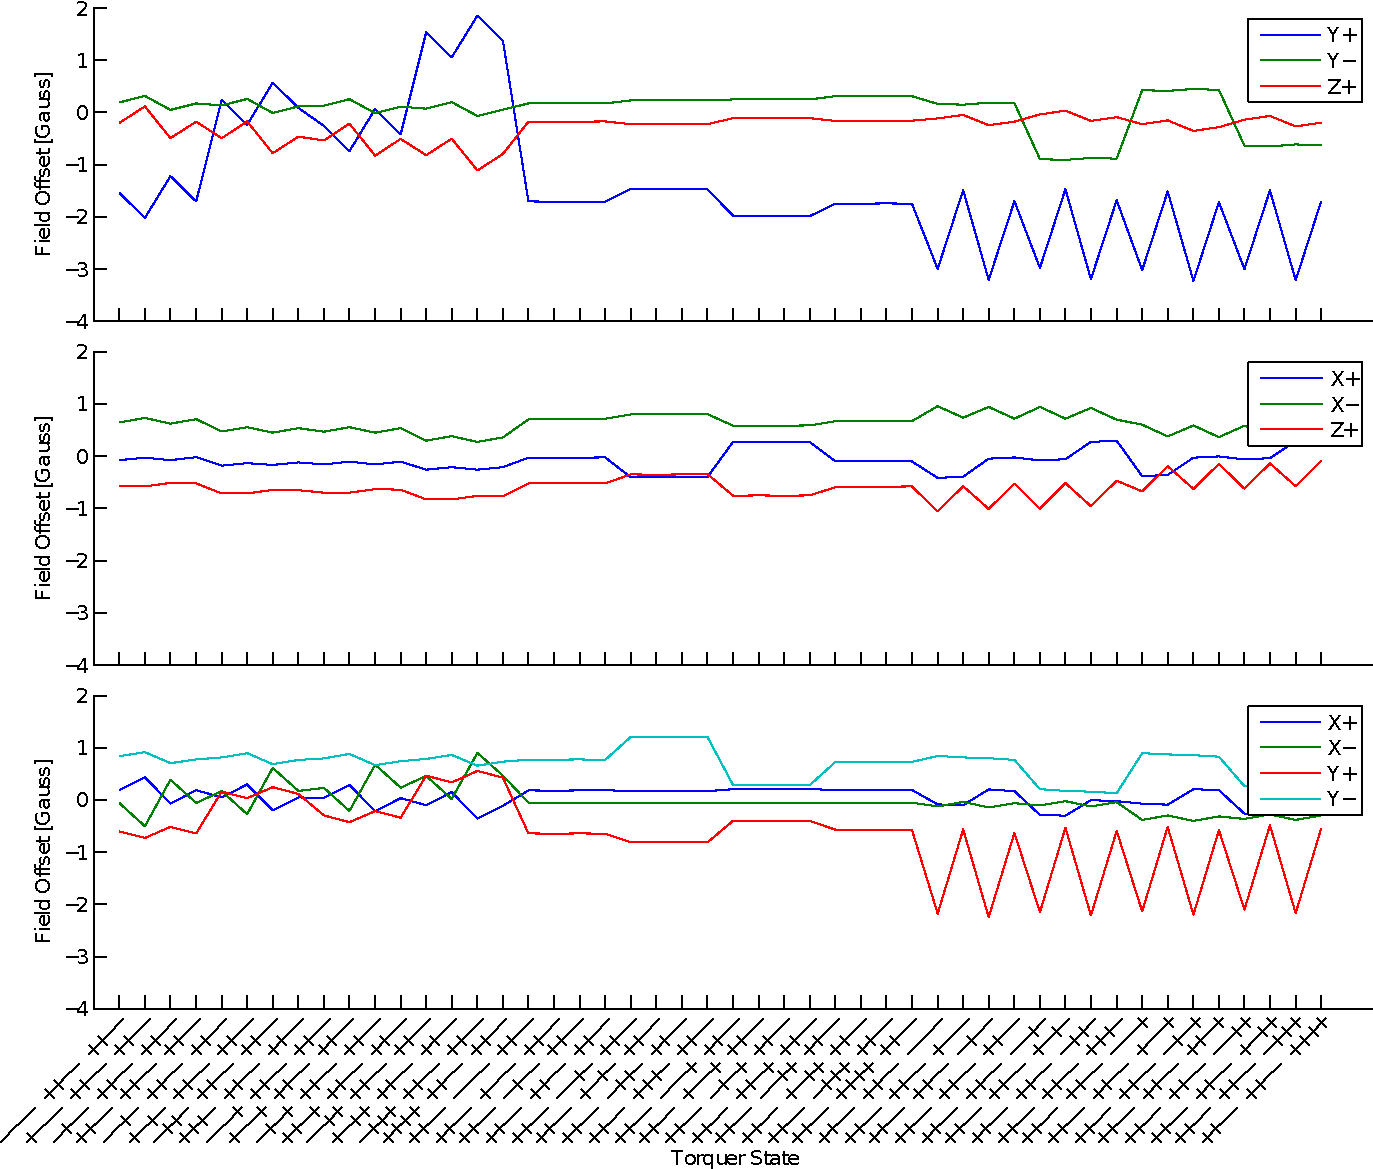
\includegraphics[width=\linewidth]{board-offsets}
    \caption{Board offsets}
    \label{fig:b-offset}
\end{figure}


The magnetic field of the earth ranges from 0.3 to 0.6 Gauss\cite[pp.~114]{Wertz}. In order to measure the attitude of the \ac{ARC} to within {\textpm5\textdegree} the Earth's magnetic field must be measured with an error of less than 26~mGauss. This means that the offsets from the torquers must be known with an accuracy of at least 26~mGauss. 

Because of the nature of the dipole magnetic field, the offsets measured by each magnetometer are unique to each magnetometer and torquer combination. Some torquers have only a small effect on each magnetometer and some have a much larger effect. \Cref{fig:b-offset} shows the magnetic field offsets with the torquers in various states. 

\Cref{fig:b-offset} shows the necessity of torquer compensation. There are large variations in the measured magnetic field due to the torquers changing state some are greater than 1~Gauss. Without torquer compensation the magnetic field from the torquers would completely overwhelm the torquers and make attitude determination impossible. What \Cref{fig:b-offset} does not show is how repeatable the offsets are which determines if compensation is possible.


\subsection{Torquer Repeatability}

\begin{figure}[!ht]
    \centering
    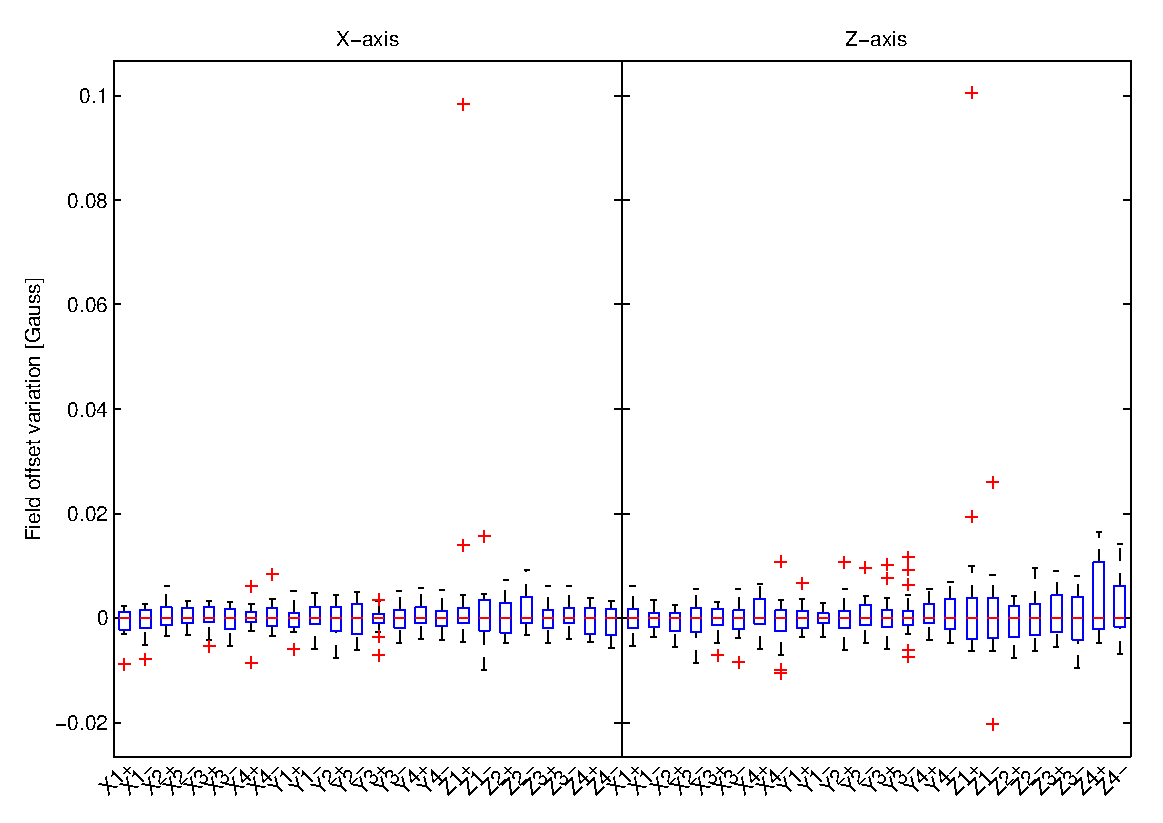
\includegraphics[width=\linewidth]{torqueOffsets}
    \caption{Box Plot from torquer offset test}
    \label{fig:tqoff}
\end{figure}

The torquer compensation method depends on the torquer offsets being repeatable. If the offsets are not very repeatable then the offsets will induce errors in the measured field. \Cref{fig:tqoff} shows a plot of the torquer offsets. The plot shows the offsets of the torquers when they are polarized in each direction. The offset for both of the magnetometer axes are shown. The offset values are normalized to show deviation from the median for better comparison. The maximum offset variation in \cref{fig:tqoff} is 20 mGauss.


%The offset variations shown in \cref{fig:tqoff} are all less than the maximum error from \cref{fig:tqerr}. This is likely because the maximum offsets did not occur all at the same time.

The plot in \cref{fig:tqoff} was generated using the code in \cref{lst:tqoff}. To create the plot each torquer was flipped 20 times in each direction. After each flip a magnetometer calibration was done to get the offset values. (more description to follow when I find the code again)

\begin{lstlisting}[style=code,caption={Code to measure torquer repeatibility for the Y+ axis},label={lst:tqoff},language=Matlab]
%TODO: find the code that I used to make the plot...
\end{lstlisting}


\section{Magnetometer Verification}

There are several steps to the magnetometer on a \ac{SPB} calibrated and verified. First the board is tested separate from the rest of the CubeSat. Next the \ac{SPB} is attached to the CubeSat and the torquer compensation routine is run to calculate the torquer offsets. Finally the compensation values are transfered to the \ac{ACDS} board and the compensation is verified.


\subsection{Initial Verification}

The magnetometer verification is done using the Helmholtz cage. A calibration is run on a board separate from the CubeSat. The calculations are done on the calibration coefficients so that they can be compared to the datasheet values to check if the magnetometers are preforming as they should. Problems are often caused by bad solder joints which can cause one or more axis to be unresponsive.

\begin{lstlisting}[style=code,caption={\ac{SPB} verification},label={lst:vspb},language=Matlab]
spbMag('X+','COM3',9600,-95.3,1);
\end{lstlisting}

\Cref{lst:vspb} shows how to verify the X+ \ac{SPB}. This will run a calibration on the magnetometer and compare the calibration values to datasheet parameters. The first argument is the address of the \ac{SPB} board this can be a symbolic address, as shown, or a numeric address (still in string form). The second and third arguments define the COM port and baud rate respectively of the serial port to use to connect to the microcontroller attached to the \ac{SPB}. The fourth and fifth parameters are the gains for the amplifier and \ac{ADC}. The amplifier gain is only used to get the expected scale factor for the magnetometer but the \ac{ADC} gain also sets the gain of the \ac{ADC} while the measurements are being taken.

\begin{lstlisting}[caption={\ac{SPB} verification results},label={lst:vspb-res},language=verbatim]
TODO: run command and collect ouput
\end{lstlisting}

\Cref{lst:vspb-res} shows the output from the \ac{SPB} verification. The calculated datasheet parameters are shown along with pass or fail depending on if the values are within the maximums specified by the datasheet.


\subsection{Torquer Compensation}

The torquer compensation for the X+ \ac{SPB} is shown in \cref{lst:tq-comp-gen}. The arguments to \lstinline[style=code,language=Matlab]$calall$ are the same as those for \lstinline[style=code,language=Matlab]$spbMag$ except this time a rotation matrix is passed that rotates from the Helmholtz cage axis to the \ac{SPB} axis.

\begin{lstlisting}[style=code,caption={Torquer compensation for the X+ \ac{SPB}},label={lst:tq-comp-gen},language=Matlab]
a = [0 0 1;-1 0 0;0 1 0];
cor=calall('X+','COM3',9600,-95.3,1,a);
\end{lstlisting}

The \lstinline[style=code,language=Matlab]$calall$ function internally calls \lstinline[style=code,language=Matlab]$tCal$ three times. Each time the X, Y or Z torquers are flipped to generate a partial calibration. Once the calibrations are complete the calibrations are combined to get one data set for all torquers.

\subsection{Compensation Testing}

The torquer compensation is tested using the \lstinline[style=code,language=Matlab]$tCalTstFull$ function. The function runs the Helmholtz Cage through a field sequence and takes measurements at each point. During the process a random torquer is flipped every 10 data points. The measurements are corrected, in Matlab, using the compensation data set and compared to the expected field. A typical plot of the data is shown in \cref{fig:tqtst}. The RMS error is also calculated for the data set so the effectiveness of the torquer compensation can be compared to the calibration without torquers.

\begin{lstlisting}[style=code,caption={Running torquer compensation test for the X+ \ac{SPB}},label={lst:tCalTst},language=Matlab]
a = [0 0 1;-1 0 0;0 1 0];
tCalTstFull('X+',cor,'COM3',57600,-95.3,1,a);
\end{lstlisting}

\begin{figure}[!ht]
    \centering
    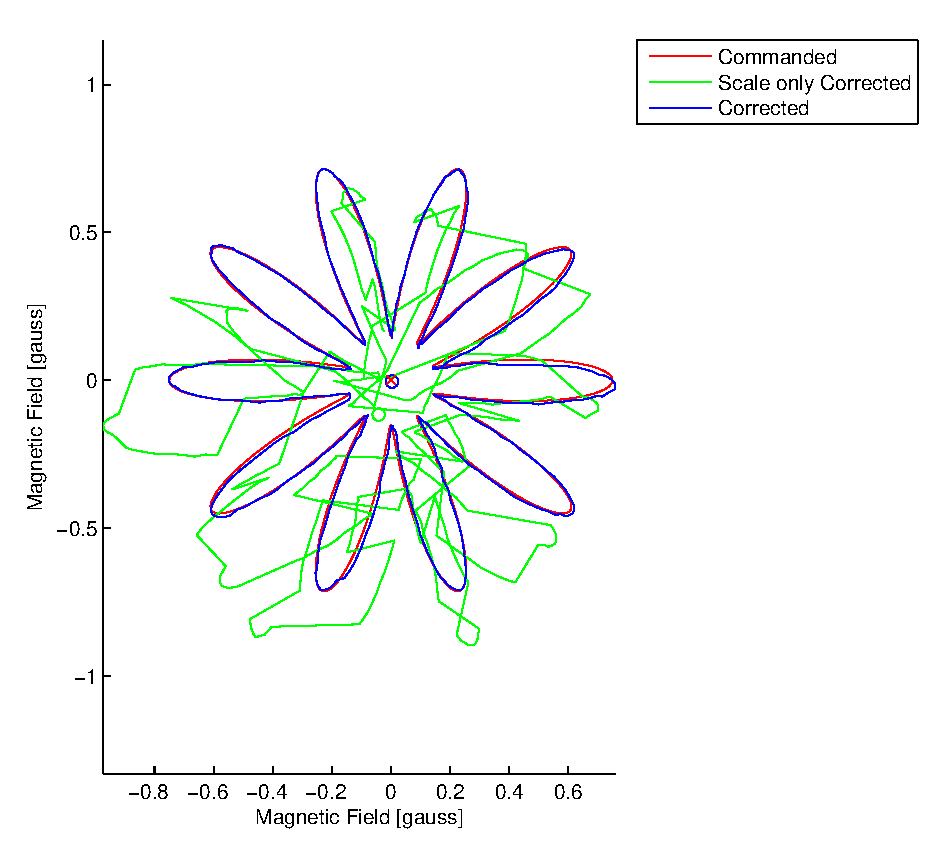
\includegraphics[width=\linewidth]{torqueCalTst}
  \caption{A torquer compensation test showing that the correction provides a large amount of improvement over the uncorrected values}
    \label{fig:tqtst}
\end{figure}

\Cref{lst:tCalTst} shows how to run the \lstinline[style=code,language=Matlab]$tCalTstFull$ function. The first argument to the \lstinline[style=code,language=Matlab]$tCalTstFull$ function is the address of the \ac{SPB} to use. The address can be specified as a number or, more continently, as a symbolic name that resolves to the correct address. The seccond argument is the correction that was previously calculated using the calall function. The third and fourth arguments are the serial port and buad rate to use to talk to the CubeSat. The fifth argument is the gain of the amplifier on the \ac{SPB} this is not really used for the calibration test because the gain is factored into the correction data. The 6th argument is the \ac{ADC} gain, this gain has already been factored into the calibration but it must be set correctly in the \ac{ADC} for the test to work properly. The last argument is the rotation matrix  The function needs a rotation matrix to transform from \ac{SPB} coordinates to Helmholtz cage coordinates. The code generates the magnetic field and plots the results in the \ac{SPB} plane.

\begin{figure}[!ht]
    \centering
    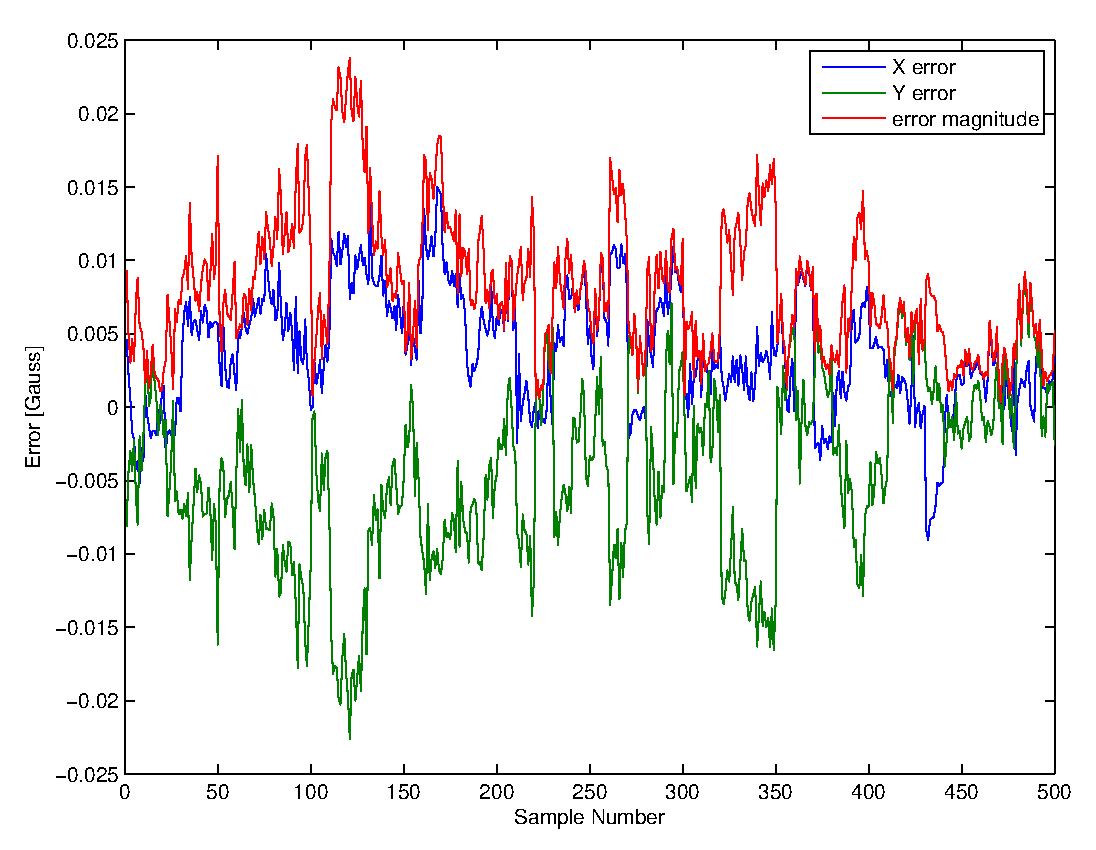
\includegraphics[width=\linewidth]{torqueCalTst-err}
    \caption{Graph showing a torquer compensation error plot}
    \label{fig:tqerr}
\end{figure}

\Cref{fig:tqerr} shows the error for the torquer compensation test. The RMS error for the compensated data is 9 mGauss. The maximum error is 24 mGauss. On a 300 mGauss field a 24 mGauss error will cause an angular error of \textpm5\textdegree. The addition of the torquers causes an increase in the RMS and maximum error.
%This can be seen by comparing \cref{fig:tqerr} with \cref{fig:magerr}. In \cref{fig:tqerr} steps in the error are seen as torquers are flipped whereas in \cref{fig:magerr} the error is more consistent across the entire run.

\subsection{Compensation Data Transfer}

The compensation data set is generated in Matlab but to be used in flight it must be stored on the \ac{ACDS} board. The calibration data is stored in the flash memory on the \ac{ACDS} microcontroller. The on-board flash has the benefit of reading the same as \ac{RAM} and is also more abundant but is a bit disruptive to write. This works well in the case of the \ac{ACDS} because the data is expected to be written once but read often. The other option would be to store the data on the \ac{SD} that is used to log data. In this case the calibration data would need to be buffered in \ac{RAM} which is much more limited than the flash. 

The main flash memory is divided into sectors that are 512 bytes long. Erasing is done on a full sector so the corection data for each \ac{SPB} is stored in its own sector. The correction data is 408 bytes long the header and \ac{CRC} that are stored with the correction data take up 4 bytes leaving 100 bytes wasted. This is not a big deal as there is an abundance of flash.

Before the correction data is sent to the \ac{ACDS} it must be repackaged this is done using the \lstinline[style=code,language=Matlab]$make_cor_dat$ function. Correction data is transfered as single precision IEEE~754 floating point numbers. Because both the \ac{ACDS} processor and most of the machines commonly used to run Matlab are little endian machines, the byte order for the transfered data is little endian. It is important to note that in both ends of the transfer no effort is made to make sure that the data order is correct so this needs to be taken into account if the endianness of one of the machines changes.

The data generated with \lstinline[style=code,language=Matlab]$make_cor_dat$ is temporally stored in the \ac{SD} on the \ac{ACDS} board. The data is stored with an identifier that includes which \ac{SPB} the data is for. On the \ac{ACDS} board the data is unpacked from the \ac{SD}, reformatted slightly, and stored in the on-board flash. 

To simplify the process of generating a calibration set the \lstinline[style=code,language=Matlab]$store_all_cal$ function was written. The \lstinline[style=code,language=Matlab]$store_all_cal$ function generates correction data for all \ac{SPB} boards, sends the data to the \ac{ACDS} and tells the \ac{ACDS} to store the data in flash. 

\begin{lstlisting}[style=code,caption={Generating and sending compensation data to the \ac{ACDS}},label={lst:st-cal},language=Matlab]
cors=store_all_cal('COM3',57600,-95.3,1);
\end{lstlisting}

\Cref{lst:st-cal} shows how \lstinline[style=code,language=Matlab]$store_all_cal$ is called. The arguments are COM port, baud rate, amplifier gain, and \ac{ADC} gain which are the same as previously discussed. The compensation data for each \ac{SPB} is returned in a cell array so that compensation testing can be done in Matlab if desired.

\subsection{Embedded Compensation Testing}

The test in \cref{fig:tqtst,fig:tqerr} only used the \ac{ACDS} embedded system to flip torquers and take measurements. To Matlab was used to do all of the calculations for the calibration. During the flight the calibration must be done on-board with the embedded system on the \ac{ACDS} board.

\begin{figure}[!ht]
    \centering
    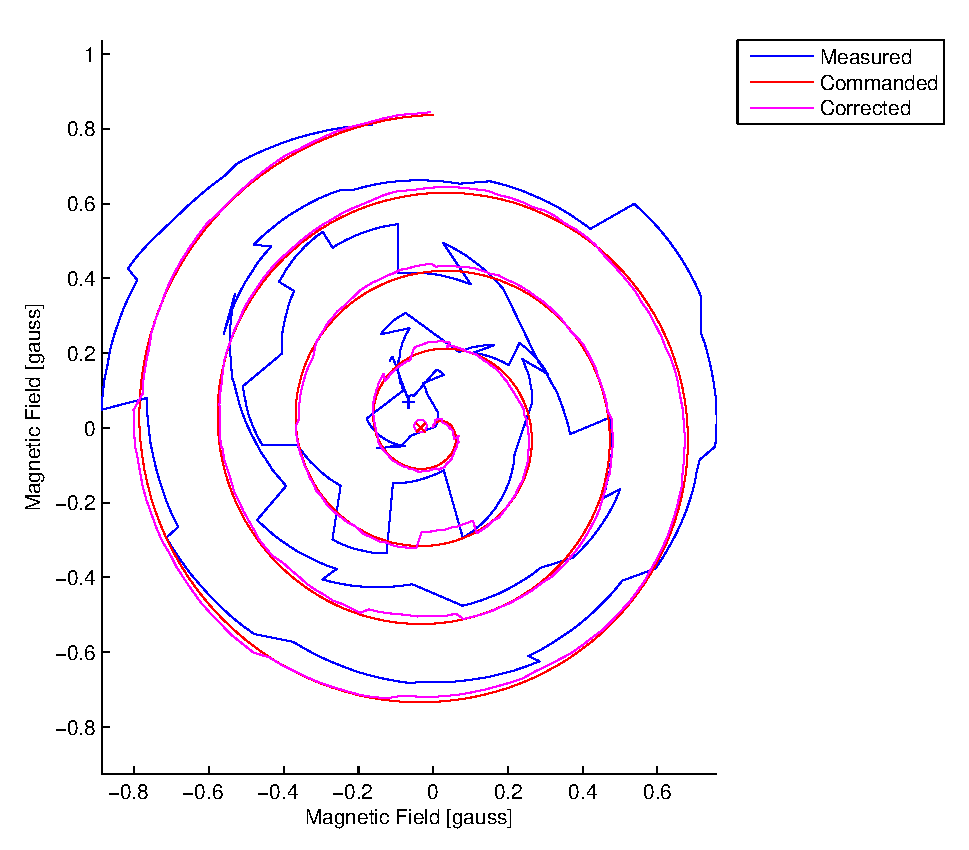
\includegraphics[width=\linewidth]{torqueCalTstMSP}
    \caption{Test of the calibration as performed by the \ac{ACDS} board}
    \label{fig:tcalMSP}
\end{figure}

\Cref{fig:tcalMSP} shows the torquer calibration test using the Y+, Y- and Z+ \acp{SPB} with the calibration performed using the embedded system on the \ac{ACDS} board. The RMS error was 14.637793~mGauss. The maximum error was 39.054539~mGauss.

\begin{figure}[!ht]
    \centering
    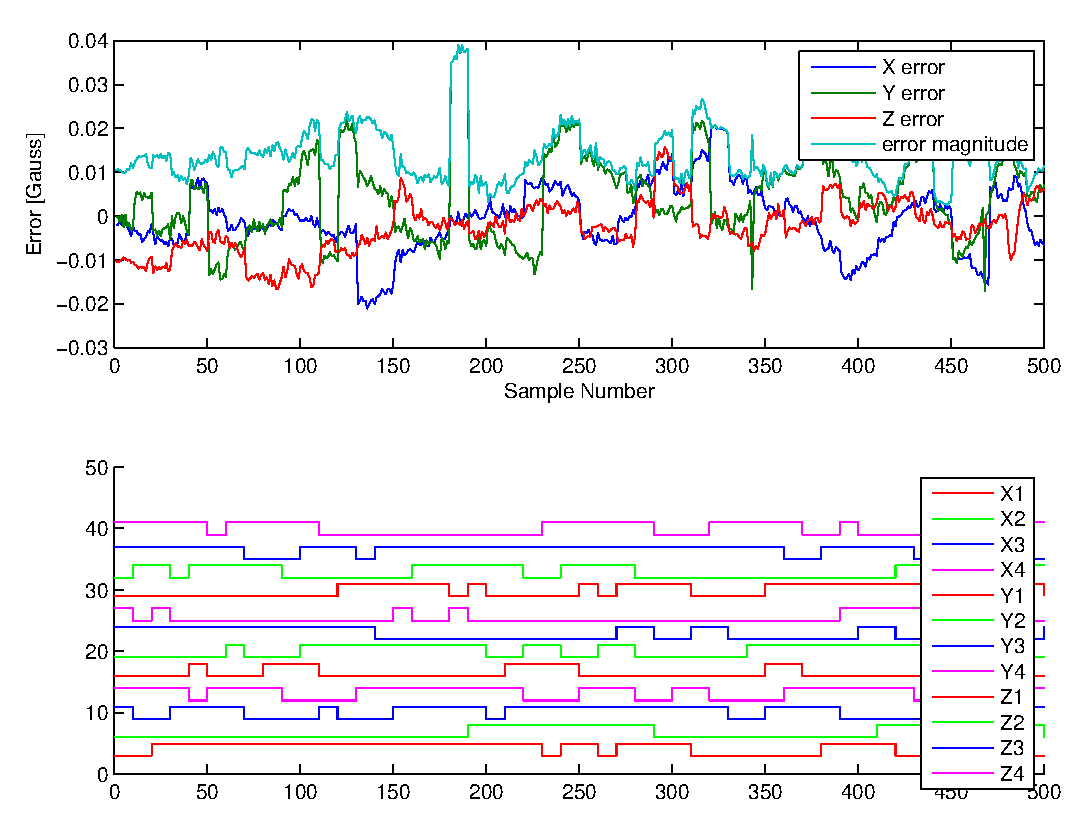
\includegraphics[width=\linewidth]{torqueCalTstMSP-err-flips}
    \caption{Error plot for \cref{fig:tcalMSP} showing torquer states}
    \label{fig:tcalMSPerr}
\end{figure}

\Cref{fig:tcalMSPerr} shows the errors for each sample as well as the torquer states during the samples. The large jumps in the errors all correspond with torquer flips.

\begin{figure}[!ht]
    \centering
    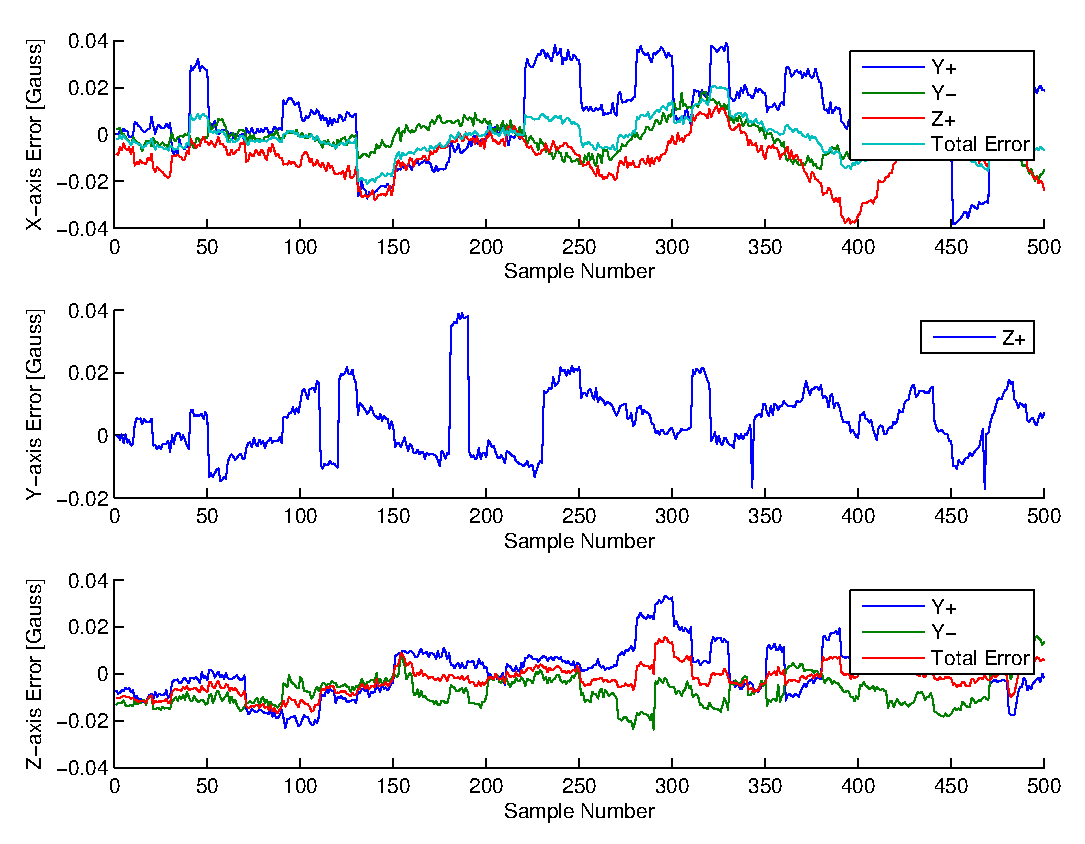
\includegraphics[width=\linewidth]{torqueCalTstMSP-err-axes}
    \caption{Plot of magnetic field errors for each axis}
    \label{fig:tcalMSPerr-axis}
\end{figure}

\Cref{fig:tcalMSPerr-axis} shows the errors from each board in each axis. \Cref{tab:tcalMSPerr} shows the RMS errors in table form.

\begin{table}[!ht]
    \centering
    \caption{Errors for \ac{ACDS} system calibration test}
    \label{tab:tcalMSPerr}
    \begin{tabular}{|c|c|c|c|}
        \hline
        &X-axis&Y-axis&Z-axis\\
        \hline
        Y+&0.018473&N/A&0.011453\\
        \hline
        Y-&0.007671&N/A&0.009875\\
        \hline
        Z+&0.013049&0.010704&N/A\\
        \hline
        Total&0.007594&0.010704&0.006483\\
        \hline
    \end{tabular}
\end{table}

\begin{comment}
X-axis errors:
    Y+ RMS error = 0.018473
    Y- RMS error = 0.007671
    Z+ RMS error = 0.013049
Total X-axis error = 0.007594

Y-axis errors:
    Z+ RMS error = 0.010704
Total Y-axis error = 0.010704

Z-axis errors:
    Y+ RMS error = 0.011453
    Y- RMS error = 0.009875
Total Z-axis error = 0.006483
\end{comment}

\clearpage
\section{B-dot controller simulations}

To verify the B-dot algorithm the \ac{ACDS} is placed in the Helmholtz cage and a rotating field is generated. The minimum rotation rate of the magnetic field that will cause a rotation rate is calculated by starting with \cref{eq:bdot-cross}

\begin{equation}
    \dot{\vec{B}} = \vec{B} \cross \omega
    \label{eq:bdot-cross}
\end{equation}

If the axis of rotation is perpendicular to the field rotation then \cref{eq:bdot-cross} becomes \cref{eq:bdot-mul}

\begin{equation}
    \dot{\vec{B}} = \left| \vec{B} \right| \cdot \left| \omega \right|
    \label{eq:bdot-mul}
\end{equation}

The B-dot algorithm equation is shown in \cref{eq:bdot-alg}.

\begin{equation}
    M_{cmd} = C \dot{\vec{B}} 
    \label{eq:bdot-alg}
\end{equation}

Substituting \cref{eq:bdot-mul} into \cref{eq:bdot-alg} and solving for $\omega$ gives \cref{eq:omega-th}. Where $M_{th}$ is the torque switching threshold for the torquers and $\omega_{th}$ is the minimum rotation rate required to flip a torquer.

\begin{equation}
    \omega _ {th} = {M _ {th} \over{ {C \left| \vec{B} \right|}}}
    \label{eq:omega-th}
\end{equation}

If a 0.5 gauss field is used and $C$ is 200 and the torquer switching threshold is $0.022 \unit{A \cdot m} ^2$ then $\omega_{th}$ is calculated as follows

\begin{equation}
    \omega _ {th} = { 0.022 \over{ {200 \cdot 0.5}}} = 0.00022 ~ \unit{rad / sec}
\end{equation}

\begin{figure}[!ht]
    \centering
    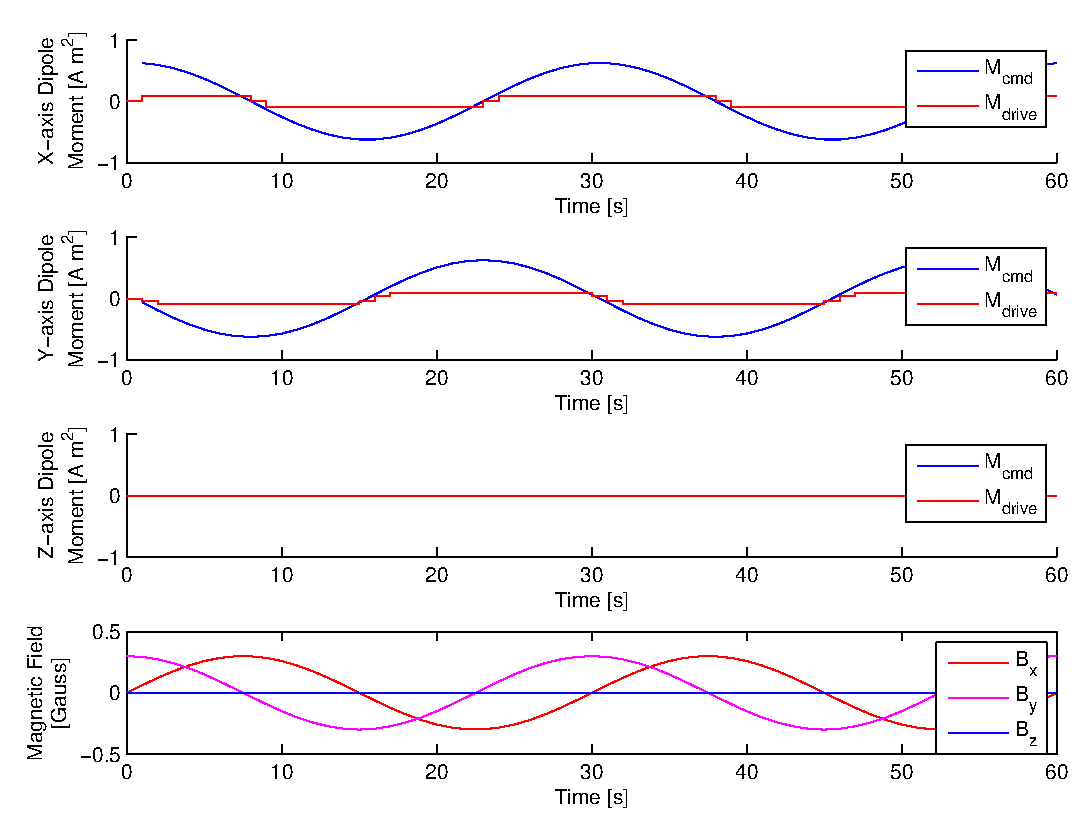
\includegraphics[width=\linewidth]{detumble-sim}
  \caption{Simulation of torquer output with spinning magnetic field}
    \label{fig:detumble-sim}
\end{figure}

%With the field set to $\omega_{th}$ a torquer should flip as $\dot{\vec{B}}$ becomes aligned with a torquer axis as the field continues to sweep the torquer will switch off.

\Cref{fig:detumble-sim} shows a simulation of the detumble algorithm in a spinning magnetic field. The field has a magnitude of 0.3~Gauss spins around the Z-axis. The plots show the magnetic dipole moment that the algorithm wants to drive and is able to drive as the magnetic field spins around.


\section{Detumble Flip Test}

\Cref{fig:detumble-test} shows the results of the detumble test. This is the same as the detumble simulation in \cref{fig:detumble-sim} except the field has been programed into the Helmholtz cage, measured by the \acp{SPB}, calculations done by the \ac{ACDS} and torquers flipped in an attempt to stop the motion.

\begin{figure}[!ht]
    \centering
    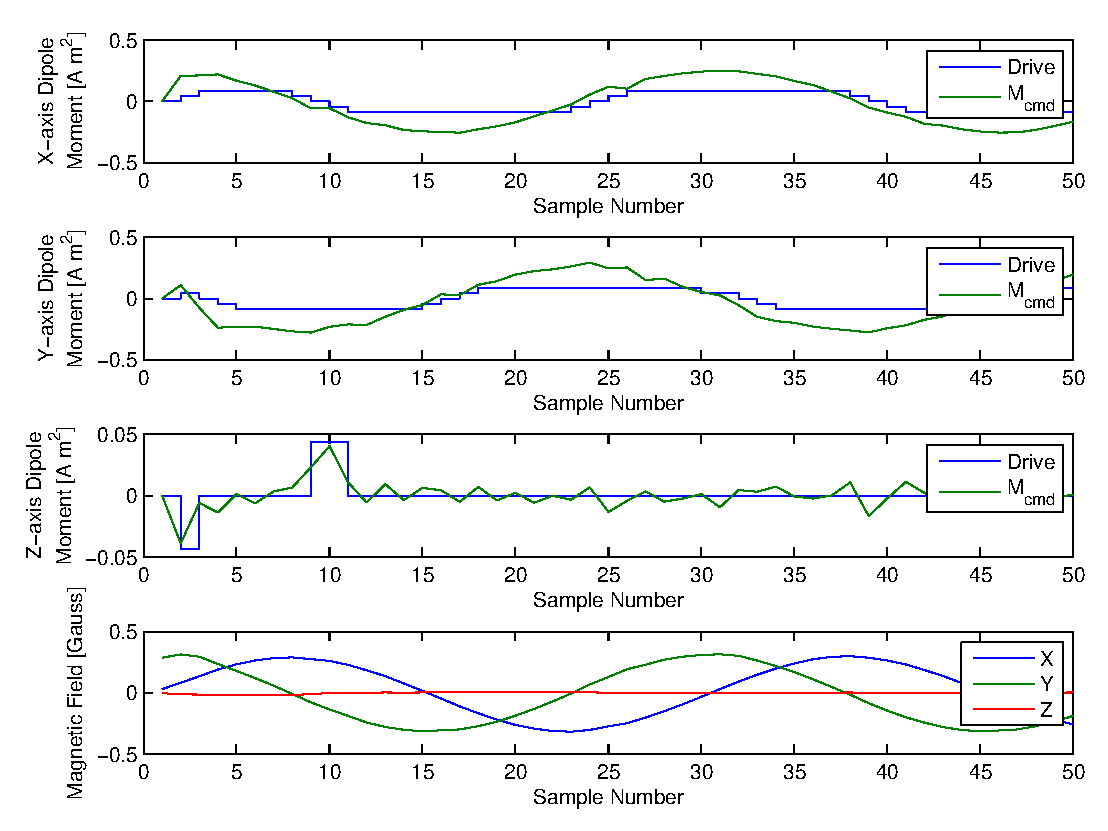
\includegraphics[width=\linewidth]{detumble-test}
  \caption{Test of the B-dot controller}
    \label{fig:detumble-test}
\end{figure}

The results in \cref{fig:detumble-test} are similar to the results in the simulation in \cref{fig:detumble-sim}. The main difference is that there are some unexpected flips in the Z-axis. This is due to noise in the magnetic field causing torquers to be flipped. It is unclear if the noise is caused by the enviornment in the Helmholtz cage or by torquer flips and imperfect torquer calibration.


